
\section{Key Findings}
\label{sec:key_findings}


The analysis of UniCL-AffSeg in the context of weakly supervised semantic segmentation reveals several key findings, which are organized below for clarity:

\subsection*{1. Local vs. Global Feature Representation}
\begin{itemize}
	\item \textbf{Strength of Swin-based UniCL encoders:} These encoders provide robust local feature representations.
	\item \textbf{Limitation:} The windowed attention mechanism restricts global semantic reasoning, which is essential for generating coherent class activation maps (CAMs).
	\item \textbf{Implication:} Future WSSS frameworks may benefit from hybrid architectures that combine local affinity-based features with global attention cues, enabling more accurate propagation of semantic information across object regions.
\end{itemize}

\subsection*{2. Affinity Maps and Multi-Scale Feature Fusion}
\begin{itemize}
	\item \textbf{Affinity maps as an alternative:} Using affinity maps instead of attention maps is effective for capturing pixel-level relationships, especially with hierarchical Swin features.
	\item \textbf{Current limitation:} The approach does not fully leverage multi-scale feature fusion due to differing spatial resolutions of stage-wise feature maps.
	\item \textbf{Future directions:} Techniques such as upsampling, feature alignment, or transformer-based fusion modules could be explored to integrate multi-scale information, improving detection of small structures and segmentation coherence for large objects.
\end{itemize}

\subsection*{3. Quality of Initial CAMs}
\begin{itemize}
	\item \textbf{Bottleneck:} The quality of initial CAMs remains a limiting factor for downstream segmentation performance.
	\item \textbf{Potential improvements:} Incorporating stronger initialization strategies (e.g., contrastive pretraining on object parts) or leveraging pseudo-label refinement techniques could enhance initial activations and lead to more accurate final masks.
\end{itemize}

\begin{figure}[thbp]
  \centering
  \setlength{\tabcolsep}{0.5pt} % adjust spacing between images
  \renewcommand{\arraystretch}{0.4}

  % Add a border using \fbox around the tabular
  \begin{center}
    \fbox{%
      \begin{tabular}{c c c}
        \textbf{Grad-CAM} & \textbf{Layer-CAM} & \textbf{Grad-CAM++} \\
        [2pt]
        % First row of images
        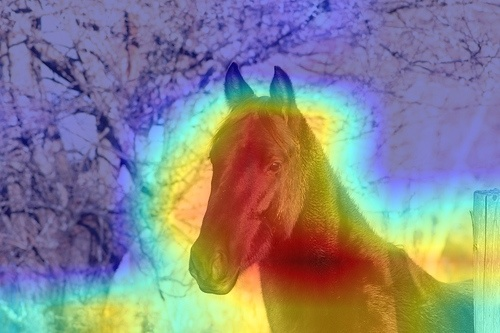
\includegraphics[width=0.18\linewidth, height=0.18\linewidth]{figures/cams/gradcam/2007_009807_12} &
        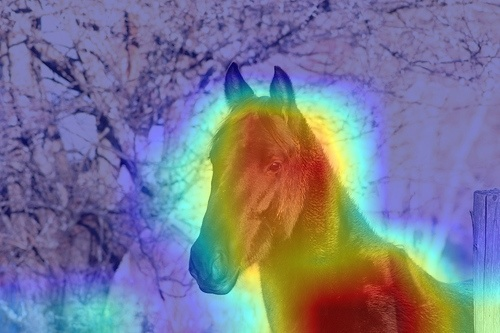
\includegraphics[width=0.18\linewidth, height=0.18\linewidth]{figures/cams/layercam/2007_009807_12} &
        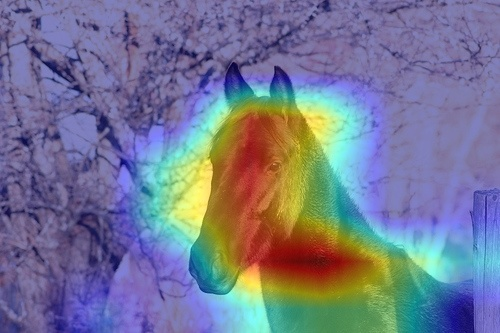
\includegraphics[width=0.18\linewidth, height=0.18\linewidth]{figures/cams/gradcampp/2007_009807_12} \\

        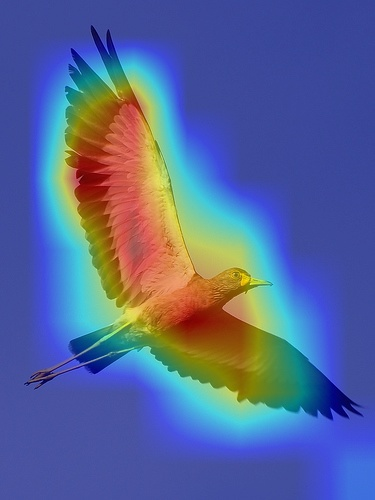
\includegraphics[width=0.18\linewidth, height=0.18\linewidth]{figures/cams/gradcam/2011_001967_2} &
        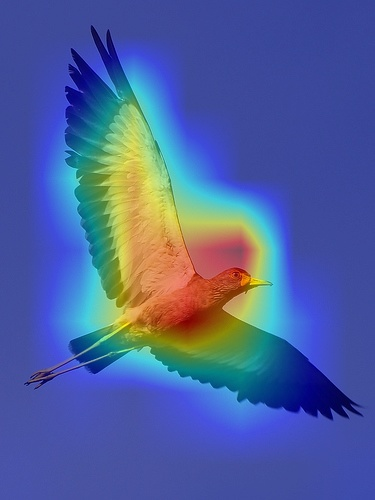
\includegraphics[width=0.18\linewidth, height=0.18\linewidth]{figures/cams/layercam/2011_001967_2} &
        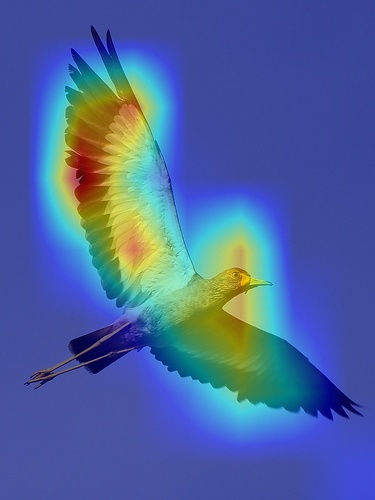
\includegraphics[width=0.18\linewidth, height=0.18\linewidth]{figures/cams/gradcampp/2011_001967_2} \\

        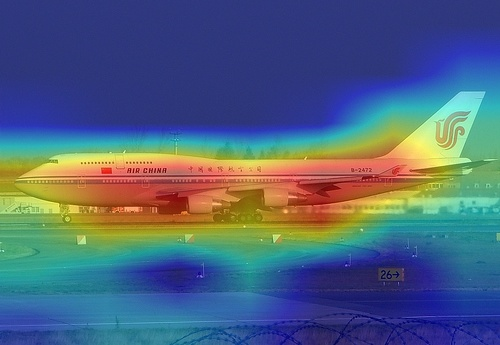
\includegraphics[width=0.18\linewidth, height=0.18\linewidth]{figures/cams/gradcam/2008_003976_0} &
        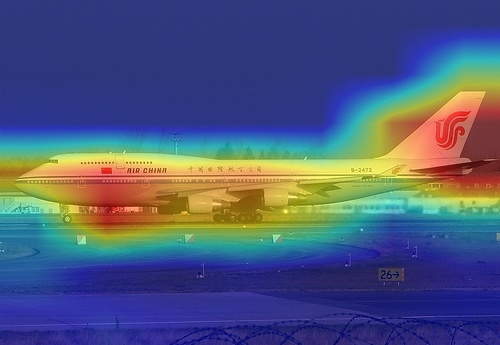
\includegraphics[width=0.18\linewidth, height=0.18\linewidth]{figures/cams/layercam/2008_003976_0} &
        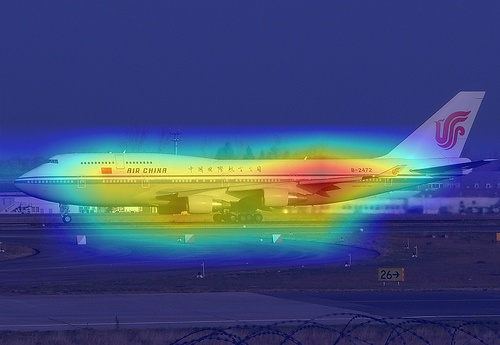
\includegraphics[width=0.18\linewidth, height=0.18\linewidth]{figures/cams/gradcampp/2008_003976_0} \\

      \end{tabular}
    }
  \end{center}

  \caption{Comparison of CAM visualization methods on the Pascal VOC dataset for single class scenario. Columns show Grad-CAM, Layer-CAM, and Grad-CAM++ respectively. Each row corresponds to a different example image.}
  \label{fig:cam_variation_singleclass}
\end{figure}


\subsection*{4. Broader Implications for WSSS Pipeline Design}
\begin{itemize}
	\item \textbf{Contrastive learning frameworks:} The results highlight the potential of frameworks like UniCL in weakly supervised settings.
	\item \textbf{Balance needed:} There is a need to balance local detail and global context for optimal performance.
	\item \textbf{General framework:} Addressing these challenges can improve segmentation performance and provide a more general approach for integrating vision-language pretraining with weak supervision in diverse visual recognition tasks.
\end{itemize}
% ...existing code...
